\documentclass{article}
\usepackage{cite}
\usepackage{graphicx}
\usepackage{listings}

\usepackage{color}
\definecolor{gray}{rgb}{0.4,0.4,0.4}
\definecolor{darkblue}{rgb}{0.0,0.0,0.6}
\definecolor{cyan}{rgb}{0.0,0.6,0.6}
\definecolor{red}{rgb}{0.8,0.0,0.2}
\definecolor{pink}{rgb}{0.8, 0.2, 0.8}
\definecolor{green}{rgb}{0.0, 0.8, 0.2}

\lstset{
  basicstyle=\ttfamily,
  columns=fullflexible,
  showstringspaces=false,
  commentstyle=\color{gray}\upshape
}

\lstdefinelanguage{XML}
{
  morestring=[b]",
  %morestring=[s]{>}{<},
  morecomment=[s]{<?}{?>},
  morecomment=[s]{<!--}{-->},
  stringstyle=\color{red},
  identifierstyle=\color{darkblue},
  keywordstyle=\color{pink},
  commentstyle=\color{green},
  morekeywords={xmlns,version,type, ToM, name, operator, value, probability}% list your attributes here
}


\begin{document}

\title{Extending Believable Agent Frameworks with Predicate
  Logic Dialogue Generation}
\author{Kaylen Wheeler}

\maketitle

\begin{abstract}

Despite advances in graphics, physics, and AI, modern video games are
still lacking in believable social simulation.  Story, dialogue, and
character behaviour are more often scripted than allowed to emerge
dynamically.  The more complex and interactive stories in modern games
may allow the player to experience different paths in dialogue trees,
but such trees are still required to be manually created by authors.
Recently, there has been research on methods of creating emergent
believable behaviour [CITE facade, fatima, acton, etc.], but these are
lacking true dialogue construction.  Because the mapping of natural
language sentences to meaningful computational representations
(logical forms) is still an unsolved problem [CITE Zettlemoyer], it
may be best to represent inter-character dialogue as logical forms.
The proposed thesis will extend an existing believable agent
framework with a predicate logic-based dialogue module that will
allow for true construction and interpretation of dialogue by
non-player characters.

\end{abstract}

\section{Introduction}

Throughout the history of video gaming, the majority of efforts to
increase believability have focused on advancement in graphics and
physics, powered largely by advances in computer hardware.  Modern
games often have near-photorealistic graphics and highly believable
physical simulation.  However, advances in AI, although present, have
not added much to believabilty.  Rather, developments in game AI are
focused on providing challenging and interesting gameplay by creating
agents that can either cooperate or compete with the player.  Such
agents, although effective in creating entertaining gameplay, fail to
create believable characters, specifically with regards to social
behaviour.

In addition to social behaviour, the ability to generate dialogue
dynamically is also lacking.  Modern games which are praised for their
complex dialogue systems, such as the \emph{Mass Effect} series [CITE Mass
  Effect] do not in fact have their characters generate dialogue, but
rather select from pre-written (and voiced) dialogue based on certain
conditions.  Even experiments in interactive drama such as Facade
[CITE facade] rely on complex ways of selecting from a set of existing
dialogue acts.  Facade is a highly variable game experience taking
only about 20 minutes to play through and consisting of a very limited
environment (a single room with one player character and two NPC's), and
yet several hundred thousand lines of code were written of handle all
possible dialogue acts\cite{Mateas}.  Clearly, such an approach is not
scalable to open world, multi-agent environments.

Believable agent frameworks are already in place which simulate
emotional and social interactions.  These systems allow for autonomous
agents to form goals based on their current emotional state and social
relations, and perform actions to satisfy those goals.

The proposed thesis will involve the implementation of an extension dialogue module
to FAtiMA\cite{Mascarenhas}, an existing believable agent framework.
Currently, the agents in FAtiMA are limited to selecting from an
existing finite set of actions to perform based on their goals and
current state.  Using the same goals and current state, the new dialogue
module would allow agents to perform not only action selection, but
action construction, creating arbitrary logical expressions to
communicate with other agents.  Additionally, the module will allow for
the interpretation of such logical expressions to affect the current
state of an agent.

\section{Background and Previous Work}

This thesis will involve the synthesis of both Believable Agent
Frameworks (abbreviated here as BAF) and Natural Language Processing
(NLP).  This section will provide background and previous research
from each of these areas.

\subsection{Believable Agent Frameworks}

A BAF is any framework that simulates the social and emotional
behaviours of humans in a believable way.  The term ``Believable'' is
difficult to define because it is subjective by nature.  However, it
is often suggested that believability is not truly an attempt to fool
the user into actually believing what is presented; it is rather an
attempt to allow the user to willingly suspend disbelief. \cite{Acton2009}

A well-known attempt to create more believable narrative and gameplay
is the Facade
project\cite{Mateas}.  Facade is a one-act interactive drama with a
natural written language interface.  The player takes on the role of a
character visiting a married couple, and is able to converse in
real-time with the other two characters by typing natural language
text.

Although Facade was created to select appropriate responses to many
situations, each of these responses was hand-authored.  Additionally,
natural language input from the user was not intrepreted to its
fullest possible extent by the program.  Rather, surface text
processing was used which searched user input for a number of key
words and phrases and mapped it to one of a finite, pre-defined set of
discourse acts. \cite{Mateasa}  In some ways, Facade can be considered
similar to dialogue trees in games such as \emph{Mass Effect}, but with an
interface that gives the illusion of natural language interaction.

Some of the creators of Facade were also involved in the
creation of the ``Comme il Faut''(CiF)\cite{Mccoy2010}, a social AI
system.  The intention of CiF was to provide a ``system for authoring playable social
models''\cite{Mccoy2010}.  Rather than authoring dialogue trees, which
the authors called ``burdensome''  and ``highly constrained'', the
Social AI System  would allow the authoring of a ``space of possible
stories''.  Through the definition of social and cultural rules that
can be applied to a given social state, believable social behaviour is
allowed to emerge.

CiF was used to implement the game \emph{Prom Week} [TODO: Cite the
  game itsetf?].  \emph{Prom Week} pioneered what the creators termed ``Social
Physics''\cite{Mccoy2011} -- intuitive rules of social
interaction that could guide the user's gameplay toward accomplishing
the game's goals, similar to how physics are used in many puzzle
games.  However, like Facade, and despite its advanced modelling of
social and emotional phenomena, the dialogue is still composed of a
finite number of templates that are selected in the appropriate
situations.

A more easily accessible (in terms of source code) and more modular
BAF is the FearNot Affective Mind Architecture (FAtiMA)
\cite{Mascarenhas}.  FAtiMA was developed initially as an engine for
\emph{FearNot!}[TODO: Cite fearnot game?], a serious game aimed at
teaching school children between ages 8 and 12 how to deal with being
bullied.

FAtiMA has a number of modules, each based around modelling aspects of
believable agents.  These include modules for modelling Theory of
Mind\cite{Marsella}, memory, emotional intelligence, dialogue, and
others.  It also has the ability to be easily extended by adding new
modules.  This feature allows different models of the same phenomena
to be implemented and tested for validity within the same framework
(e.g. evaluating different theories of emotion appraisal for their
believability).

In terms of dialogue, FAtiMA currently has a module that maps Theory
of Mind (ToM) - related goals to pre-defined discourse actions.  Theory of
Mind goals differ from other goals in that they seek to affect the
state of another agent's beliefs rather than the state of the world
itself.  These dialogue acts, however, are not creted dynamically and
must be manually authored and explicitly mapped to corresponding agent
goals.


\subsection{Natural Language Processing}

Natural language processing is still an ongoing area of research.  Recent
developments have lead to more advanced search engines and data mining 
techniques, as well as computer-aided natural language translation.  However,
the problem of mapping natural language sentences to meaningful forms that can
be effectively interpreted by a computer is still a very open problem.

Zettlemoyer \cite{Zettlemoyer2004} has conducted some interesting research
on the topic of mapping natural language sentences to lambda calculus
expressions, which can be easily represented as sentences in
first-order logic.  His research makes use of combinatory categorical
grammars (CCG) \cite{Steedman2003} generated by advanced machine
learning techniques in order to parse sentences of various natural
languages.

An example of a mapping of natural language to lambda calculus is
demonstrated below.  Here, the sentence ``What states border Texas?''
is mapped to an equivalent lambda expression.  The expression takes as
a parameter a single unbound variable \emph{x}, which must satisfy the
condition of being a state and bordering texas.  When the expression
is used as a query to a knowledge base, \emph{x} unifies with all
values that satisfy both conditions.

\begin{figure}[h!]
\begin{center}
{
\center ``What states border Texas?''}

\[
 \lambda x.(state(x) \wedge  border(x,Texas))
\]
\[
 x = \{NewMexico, Oklahoma, Arkansas, Louisiana\}
\]

\end{center}
\end{figure}

Although the specifics of the theory and implementation are beyond the
scope of -- and likely of little relevance to -- this proposal, the
important realization is that natural language sentences can be
transformed into these forms, as well as the fact that software exists
that can accomplish this transformation[TODO: Reference Openccg?].
Using software to translate logical expressions into natural language
could allow the creation of language-independent dynamic dialogue
systems that can be easily localized into different languages.


\section{Problem Description and Proposed Solution}

Although many of the Believable Agent Frameworks researched so far
have had extensive flexibility in the use of authored dialogue, the
fact still remains that the dialogue must be authored.  For each
dialogue act, its representation (i.e. words used in the dialogue) as well as
each of its effects on the world or other agents must be explicitly
defined.  Additionally, explicit mappings between agents' states or
goals to dialogue actions must be provided (e.g. the goal to make
another character laugh must explicitly relate to the ``tell joke''
action).

The proposed solution is to create a system that alleviates the need
to explicitly author dialogue acts.  Rather than providing a set of
mappings between domain-specific dialogue acts and goals, a
domain-independent module will be created that constructs dialogue
acts to match goals.  The system will be implemented as an extension
to FAtiMA's existing dialogue system.

FAtiMA uses knowledge bases to represent both the state of the world
and the beliefs of individual agents.  These knowledge bases have
capabilities similar to first-order logic systems.  Rather than
generating natural language dialogue, first-order logic expressions
will be created to accomplish the goals that have been specified by
the agents.

If possible, the solution may also include natural language
``rendering'' and ``de-rendering'' modules.  These would allow logical
expressions to be converted to and from natural language sentences.
This is not necessary in the implementation, but may be included if
time allows in order to demonstrate how natural language could further
improve believability.

\subsection{Illustrative Example}

To understand the differences between authoring and generating
dialogue actions, an example will be provided.  This represents a
hypothetical scenario involving two characters -- Good Guy and Bad
Guy, who complement and insult one another.  Three main components are
defined for each character -- goals, action tendenceies, and
actions.  These defined in pseudocode, visible in figure
~\ref{example_goals}.

\begin{figure}[h!]
  
  \begin{center}
    \large{Good Guy}
  \end{center}
  
  Goals:
  \[
  isHappy(target)
  \]

  Action Tendencies:
  \[
  \lambda x.\lambda p.(knows(self, mother(x,self) \wedge good(p) \wedge p(x)) \mapsto isHappy(self))
  \]
  \[
  \lambda x.\lambda p.(knows(self, mother(x,self) \wedge \neg bad(p) \wedge p(x)) \mapsto \neg isHappy(self))
  \]

  Actions:
  \[
  complement(target) \mapsto knows(target, isHandsome(target))
  \]

  \[\]

  \begin{center}
    \large{Bad Guy}
  \end{center}
  
  Goals:
  \[
  \neg isHappy(target)
  \]

  Action Tendencies:
  \[
  \lambda p.(knows(self, good(p) \wedge p(self)) \mapsto isHappy(self))
  \]

  Actions:
  \[
  \lambda x.(insultMother(target) \mapsto knows(target, mother(x, target) \wedge
  isFat(x))) 
  \]
  
  \[\]

  \begin{center} \large{General Knowledge} \end{center}

  \[
  good(isHandsome)
  \]
  \[
  good(isThin)
  \]
  \[
  bad(isUgly)
  \]
  \[
  bad(isFat)
  \]

  \caption{An example of goal, action tendency, and action
    specification for two agents.  The left side of the $\mapsto$ symbol
    represents the preconditions in the case of action tendencies and
    action definitions in the case of actions.  The right side
    represents the effect.  The variables \emph{self} and
    \emph{target} are references to the agent's self and another in
    the environment.  Unbound variables are introduced with $\lambda$-notation.}
  \label{example_goals}

\end{figure}

Goals represent states that the agents are striving to achieve.  In
the case of Good Guy, his goal is that \emph{target}(i.e. Bad Guy)
should be happy.  Bad Guy's goal, on the other hand, is that
\emph{target}(i.e. Good Guy) should not be happy.

Action tendencies represent how agents act when faced with certain
situations.  The particular situations illustrated here involve
knowledge, and are defined with the \emph{knows} predicate.  (At the
moment, FAtiMA supports action tendencies in response to events.  To
support this dialogue system, it will need to be extended to analyze
changes in knowledge bases.)  For Good Guy's action tendencies, an
unbound variables \emph{x} and \emph{p} are introduced.
The variable \emph{x} unifies with \emph{self}'s mother, while \emph{p}
unifies with some predicate, which is \emph{good} or \emph{bad}.
The results (after the $\mapsto$ symbol) are either happiness or uhnappiness.  Thus, the
action tendencies for Good Guy can be described as ``If I know something
good about my mother, I am happy.'' and ``If I know something bad about my mother, I
am not happy.''.  Similarly, Bad Guy's action tendency is ``If I know
something good about me, I am happy.''.

A finite set of actions is defined, representing potential effects
that agents may have on the world.  A continuous partial-order planner
\cite{Paiva2005, Russell2003} is used to construct plans composed of
sequences of actions that achieve the agent's goals.  However, the
actions in the sequence may only be selected from a finite,
pre-defined set of actions.  The goal of this thesis will be to allow
for actions to be constructed from the goal they are trying to achieve.

\subsubsection{Example Plans}

Two examples are shown in figures ~\ref{plan_selection} and ~\ref{plan_construction}.
The first example shows an example of how an agent's plan would be
constructed if using action selection (the current method), while the
second shows how a plan might be created using action construction
(the proposed method.  In the example scenario, Bad Guy is attempting
to fulfill the goal of making some target (Good Guy) feel unhappy.

For each figure, the first few steps are the same.  We'll start with
figure ~\ref{plan_selection}.  First, the goal of causing
unhappiness is identified.  Using knowledge about the Good Guy's
action tendencies, Bad Guy is able to discern that Good Guy would
feel unhappy if he knew something bad about his mother.  Bad Guy's existing
set of actions are then analyzed to determine if any of them can
cause Good Guy to know something bad about his mother.  Because the
predicate \emph{isFat} is idenified in the general knowledge base as
being \emph{bad}, the action \emph{insultMother} is chosen to satisfy the
goal.

The important difference in ~\ref{plan_construction} is that Bad Guy's
set of actions are not analyzed for a solution.  Instead, an action
is constructed.  Bad Guy is able to construct logical statements
that will change Good Guy's knowledge state.  In this case, the posisble
statements involve bad things said about Good Guy's mother.  Using
an expression-construction algorithm (which is yet to be determined),
Bad Guy is able to construct a variety of expressions which have the
desired effect.  In this case, the expressions constructed equate to
``Your mother is fat.'' and ``Your mother is ugly.''.  In the current
system, the fat and ugly insults would have had to be separately
authored.  The proposed system will enable dynamic and varied
dialogue construction for any knowledge-related goals.

\begin{figure}[h!]
  
  \begin{center}\large{Action Selection}\end{center}

  Goal:
  $$
  \neg isHappy(target)
  $$

  Knowledge about target:
  \[
  \lambda x.\lambda p.(knows(self, mother(x,self) \wedge good(p) \wedge p(x)) \mapsto isHappy(self))
  \]
  \[
  \lambda x.\lambda p.(knows(self, mother(x,self) \wedge bad(p) \wedge p(x)) \mapsto \neg isHappy(self))
  \]

  Planner infers that the effect:
  \[
  \neg isHappy(target)
  \]

  Can be accomplished with:
  \[
  \lambda x.\lambda p.(knows(self, mother(x,self) \wedge bad(p) \wedge p(x)) \mapsto \neg isHappy(self))
  \]

  This becomes the new Goal.

  The planner analyzes the available actions:
  \[
  \lambda x.(insultMother(target) \mapsto knows(target, mother(x, target) \wedge
  isFat(x))) 
  \]

  If \emph{p} unifies with \emph{isFat}, it satisfies $bad(p)$.  The planner infers that
  the action \emph{insultMother} will have an effect identical to the goal it wants to accomplish.
  Therefore, Bad Guy's plan is to take the action:
  
  \[
  insultMother(target)
  \]

  \caption{Bad Guy's plan for insulting Good Guy's mother with action selection.}
  \label{plan_selection}
\end{figure}

\begin{figure}[h!]
  
  \begin{center}\large{Action Construction}\end{center}

  Goal:
  $$
  \neg isHappy(target)
  $$

  Knowledge about target:
  \[
  \lambda x.\lambda p.(knows(self, mother(x,self) \wedge good(p) \wedge p(x)) \mapsto isHappy(self))
  \]
  \[
  \lambda x.\lambda p.(knows(self, mother(x,self) \wedge bad(p) \wedge p(x)) \mapsto \neg isHappy(self))
  \]

  Planner infers that the effect:
  \[
  \neg isHappy(target)
  \]

  Can be accomplished with:
  \[
  \lambda x.\lambda p.(knows(self, mother(x,self) \wedge bad(p) \wedge p(x)) \mapsto \neg isHappy(self))
  \]

  This becomes the new Goal.

  There are no actions for the planner to select from.  Instead it generates speech
  actions.

  \[
  talkAction_1(me, you) \mapsto communicate(me, you, \lambda x.(mother(x, you) \wedge isFat(x)))
  \]
  \[
  talkAction_2(me, you) \mapsto communicate(me, you, \lambda x.(mother(x, you) \wedge isUgly(x)))
  \]

  Because \emph{p} can unify with anything that is \emph{bad}, it can either unify with
  \emph{isUgly} or \emph{isFat}, allowing new and interesting insults to be generated
  without the need for explicit authoring.

  Bad Guy therefore has two possible plans of action:

  \[
  talkAction_1(self, target)
  \]
  \[
  talkAction_1(self, target)
  \]

  \caption{Bad Guy's plan for insulting Good Guy's mother with action construction.}
  \label{plan_construction}
\end{figure}

\section{Design}

\subsection{Overview of FAtiMA}

Figure ~\ref{fatima_arch} shows the high-level architecture of FAtiMA.
Agents exist in the world and are able to perceive their environments
with Sensors and change their environments with Effectors.  When an event
is perceived, it is emotionally appraised.  This appraisal tells the
agent how the event should be interpreted and how it should affect its
memory, emotions, intentions, and plans.  After appraisal, the agent begins
its coping process.  Coping determines how the agent should act given the
state of its emotion and memories.

Both appraisal and coping act on two different levels -- reactive and
deliberative.  The reactive level deals with instantaneous, reflexive
actions.  These typically equate to actions that result from instinct,
such as yelling when hurt.  The Deliberative level deals with long-term
actions which require more deliberated planning.  The deliberative layers
make use of continuous planners with partial-order plans in order to
achieve goals. \cite{Paiva2005, Russell2003}

\begin{figure}[htb]

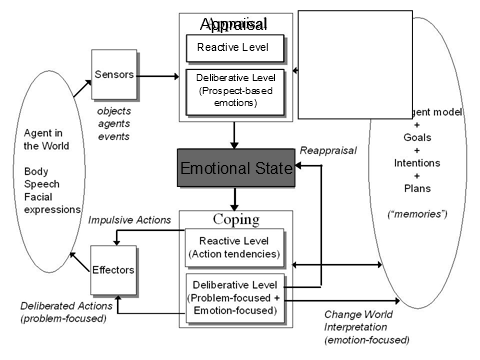
\includegraphics{Graphics/fatimadiagram.png}
\caption{FAtiMA's architecture \cite{Paiva2005}.}
\label{fatima_arch}
\end{figure}

\subsection{FAtiMA World and Knowledge Representation}

FAtiMA's planning modules construct plans that affect the world state
and agents' knowledge states.  In fact, the world state in FAtiMA is
a special case of agents' knowledge states.  The world state consists
of all knowledge that is consistent across all agents in the world.
That is, if all agents believe the same fact, it is true (the potential
philisophical implications of this view are profound, but I won't get
into that).

Figure ~\ref{xml_source_1} shows an example of how actions may be defined
for agents in FAtiMA.  This particular action is part of a simple scenario
in which the user guesses which box a coin is hidden in.  The Open action
is described here.  Its preconditions state that the target (a box) must be
on the table, another agent ([AGENT]) must be present, and be a person, and
not equal the original agent (SELF).

The next two predicates specify further preconditions relating to individual
agents.  In general, predicates specify only a name attribute, which allows
description of general facts about the world.  For instance, [target](OnTable)
specifies that the target is on the table.  However, a ToM (Theory of Mind)
attribute may be specified, which restricts the predicate to describe only
the knowledge of the selected agent.  The fifth precondition specifies ToM
to be SELF.  Therefore, while ![target](Contains, coin) would usually mean
``the target does not contains the coin'', the ToM attribute restricts it to mean
``I think do not think that the target contains the coin''.  Therefore, the
last two preconditions (which determine the outcome of the game) state that
the original agent must not think that the box contains the coin, and that
the other agent must think that it does.  The final result of taking this
action is that the original agent has the coin.


\begin{figure}[hb]
\lstset{language=XML}
\begin{lstlisting}
<Action name="Open([target])" probability="0.8">
	<PreConditions>
		<Predicate name="[target](OnTable)"/>
		<Predicate name="[AGENT](isPerson)"/>
		<Property name="[AGENT]" operator="!=" value="SELF" />
		<Predicate ToM="SELF" name="![target](Contains,coin)"/>
		<Predicate ToM="[AGENT]:SELF" name="[target](Contains,coin)"/>
	</PreConditions>
	<Effects>
		<Effect probability="1.0">
			<Predicate name="SELF(has,coin)"/>
		</Effect>
	</Effects> 
	<EffectsOnDrives>
	</EffectsOnDrives>
</Action>
\end{lstlisting}
\caption{Example of an action defined in FAtiMA's XML format.}
\label{xml_source_1}
\end{figure}

Figure ~\ref{xml_source_2} shows a specification of a goal in the same XML
format.  Like the action, the goal specifies a set of preconditions.  However,
rather than specifying effects directly, it specifies success conditions.
These success conditions allow the planner to select actions that can accomplish
the goal.  For instance, the success condition here is SELF(has,coin).  Since
this matches the effect of the action in figure ~\ref{xml_source_1}, the planner
will select that action to accomplish this goal (as long as the preconditions match).

\begin{figure}
\lstset{language=XML}
\begin{lstlisting}

<ActivePursuitGoal name="Test([target])">
	<PreConditions>
		<Property name="[target](isPerson)" operator="=" value="True" />
		<Property name="[target]" operator="!=" value="SELF" />
		<RecentEvent ToM="[target]" occurred="True"
                subject="[target]"
                action="SpeechAct"
                target="SELF"
                parameters="starttest"/>
		<Property name="[box](type)" operator="=" value="Box"/>
		<Predicate ToM="[target]:SELF" name="![box](Contains,coin)"/>
	</PreConditions>
	<SuccessConditions>
		<Predicate name="SELF(has,coin)"/>
	</SuccessConditions>
	<FailureConditions>
	</FailureConditions>
	<ExpectedEffects>
		<OnSelect drive="Affiliation" target="SELF" value="+2"/>
	</ExpectedEffects>	
</ActivePursuitGoal>

\end{lstlisting}
\caption{Example of a goal defined in FAtiMA's XML format.}
\label{xml_source_2}
\end{figure}

\subsection{Action Construction vs. Action Selection}

This thesis aims to enable action construction in this system.  In those
cases where goals are defined with success conditions that have ToM
attributes specified (i.e. when they attempt to make another agent
believe something rather than affecting the world), the planner should
not have to select from a set of pre-written actions.  Instead, actions
will be constructed as first-order logic expressions that affect the
knowledge base.

These expressions will be produced by a sender agent and received by another
receiver agent.  The receiver will interpret the expression and affect
its own knowledge base accordingly.

The specific format used for communication of first-order logic expressions,
as well as the algorithms used for action construction, have yet to be determined.

\section{Timeline}

TODO: I'll discuss this with you.

\bibliographystyle{plain}
\bibliography{references}{}

\end{document}
